\documentclass[runningheads]{llncs}

\usepackage{graphicx}
\usepackage{booktabs}
\usepackage{amsmath}
\usepackage{hyperref}
\usepackage{caption}
\usepackage{subcaption}
\usepackage[table]{xcolor}

\definecolor{bestgreen}{RGB}{0,150,0}
\definecolor{secondblue}{RGB}{200,230,255}

\title{Extended Evaluation of SnowPole Detection for Machine-Perceivable Infrastructure for Nordic Winter Conditions: A Comparative Study of Object Detection Models}

\titlerunning{SnowPole Detection: Comparative YOLO Evaluation}
 \date{\today}
\author{
Durga Prasad Bavirisetti\inst{1,2} \and
Muhammad Ibne Rafiq\inst{3} \and
Shaira Tabassum\inst{1} \and
Gabriel Hanssen Kiss\inst{1} \and
Frank Lindseth\inst{1}
}

\authorrunning{D.P. Bavirisetti et al.}

\institute{
Dept. of Computer Science, NTNU, Trondheim, Norway \and
Dept. of Computer Science, University of Gävle, Gävle, Sweden \and
Dept. of Mathematics and Computer Science, Eindhoven University of Technology, Netherlands \\
\email{durga.prasad.bavirisetti@hig.se} \\
}

\begin{document}



\maketitle
\begin{abstract}
Robust detection of roadside infrastructure such as snow poles is critical for safe autonomous navigation and infrastructure monitoring in Nordic winter conditions. Building upon our prior work that systematically benchmarked recent YOLO architectures across diverse LiDAR modalities, this extended study investigates multimodal fusion strategies for enhancing detection performance under challenging environmental conditions. We introduce a dual-branch RGBA framework that extends YOLOv9 and YOLOv11 architectures to process RGB pseudo-color LiDAR images alongside range information as an additional alpha channel. Our methodology incorporates transfer learning from pre-trained single-modality models and performs comprehensive ablation studies across attention mechanisms, modality contributions, and fusion architectures. Additionally, we propose a Merkle tree-based inference caching strategy for computational efficiency during sequential processing. Results demonstrate that RGB+Range fusion with cross-attention mechanisms improves detection accuracy by capturing complementary geometric and spectral information, while maintaining real-time feasibility. The attention ablation reveals that channel-spatial attention contributes measurably to recall improvements on low-contrast poles, and fusion architecture comparisons show that gated fusion balances accuracy and latency better than simple concatenation. Our tile-based caching approach achieves significant speedups on static scene regions with minimal accuracy degradation. These findings provide practical guidelines for deploying multimodal object detection pipelines in safety-critical winter driving scenarios.
PLEASE KEEP IN MIND, DUE TO EDGE DEVICE AS A REQUIREMENT, WE ARE ONLY LOOKING INTO SINGLE-stage OBJECT DETECTION MODELS SINCE 2-STAGE MODELS WILL BE INHERENTLY heavier.??????????
-Dont forget to look at skewness of smaller stuff like object detection models in particular...
All datasets, code, and trained models are publicly available to support reproducibility via our GitHub repository\footnote{\url{https://github.com/MuhammadIbneRafiq/Extended-evaluation-snowpole-lidar-dataset}} and the Mendeley dataset archive\footnote{\url{https://data.mendeley.com/datasets/tt6rbx7s3h/3}}.
\end{abstract}







\textbf{Keywords:} Snow Pole Detection, Object Detection, LiDAR Perception, YOLO Models, Multimodal Fusion, Localization, Nordic Winter Conditions

% \begin{multicols}{2} % Start two-column environment



\section{Introduction}

Robust detection and localization of roadside elements such as snow poles are vital for infrastructure safety and reliable autonomous vehicle operation during harsh Nordic winters. Snow poles serve as essential visual references when accumulated snow obscures lanes, curbs, and other markings. However, accurately identifying these objects is challenging due to unpredictable weather, occlusions, varying lighting conditions, and the inherent sparsity and noise of LiDAR data in real-world scenarios.

In prior work~\cite{bavirisetti2024pole}, we developed a YOLOv5s-based detection and geolocation pipeline on LiDAR signal images, establishing a baseline for this problem. Building on this, we released the SnowPole Detection dataset~\cite{bavirisetti2025snowpole}, which includes diverse annotated 360-degree LiDAR scans collected with an OS2-128 sensor mounted on an autonomous vehicle across mountainous roads, open terrain, and forested areas.

The raw point clouds were converted to panoramic LiDAR images across four modalities: Near-Infrared (Near-IR), Signal, Reflectivity, and Range. To support further experimentation, pseudo-color images were created by mapping these channels to RGB layers. Annotation was conducted in Roboflow and refined in CVAT to ensure high-quality labels. The dataset comprises 1,954 labeled samples split 70/20/10 for training, validation, and testing. Since modalities are spatially aligned, labels are consistent across channels, and the dataset is publicly available on Mendeley Data.

In this work, we present an extended version of the dataset~\cite{bavirisetti2025extended} (Mendeley Version 3), which includes the original modalities, the initial RGB combination, and five new pseudo-color configurations. While earlier results confirmed feasibility with single-channel inputs, key questions remained about how recent object detectors would perform across modalities and what trade-offs would arise in detection performance and latency.

Recent studies highlight that combining complementary sensor channels can improve detection robustness in adverse conditions~\cite{zafar2024realtime,nature2023fusion}. Motivated by this, we systematically evaluate YOLOv5s, YOLOv7-tiny, YOLOv8n, YOLOv9t, YOLOv10n, and YOLOv11n across all input configurations. Our analysis uses standard detection metrics (Precision, Recall, mAP@50, mAP@50--95) and measures inference latency on GPU and CPU hardware. To enable systematic comparison, we also introduce a composite \emph{Rank Score} metric that integrates detection accuracy and real-time performance. Our objective is to identify configurations offering the best trade-off between detection quality and inference efficiency for deployment in challenging Nordic winter environments.


\section{Related Work}

Talk about 3VL tree structures ad incremental learning with tree like data structures approach.



KEEP THIS IN MIND FOR CONSIDERING OTHER FORMS OF fusion wiht the range images
\subsection{Modality Harmonization Options}

\begin{itemize}
    \item \textbf{Convert all modalities to grayscale (8-bit).} Reduces storage and compute while retaining edge/shape cues and simplifies multi-modal alignment.\footnote{\href{https://www.geeksforgeeks.org/how-do-you-decide-whether-to-utilize-grayscale-or-colour-images-as-input-for-computer-vision-tasks/}{GeeksforGeeks: Grayscale vs.\ Color}}  
    \item \textbf{Select a single band/channel.} Keeps raw sensor dynamics for that band but discards spectral diversity; best when one channel carries dominant signal (e.g., near-IR contrast for vegetation).  
    \item \textbf{Preserve higher bit depth (e.g., 16-bit).} Maintains sensor dynamic range for subtle intensity differences at the cost of larger files and higher training requirements.\footnote{\href{https://en.wikipedia.org/wiki/Grayscale}{Wikipedia: Grayscale numerics and conversion}}  
\end{itemize}

This subsection can be dropped directly into your report to document why the script normalizes each modality to grayscale 8-bit before stacking, while also noting alternatives when richer spectral or radiometric detail is needed.

\subsection{LiDAR-Based Object Detection}

LiDAR sensors have become a core modality for autonomous perception, offering high-resolution spatial information robust to illumination changes. Early pipelines relied on voxelization and multi-view projections of point clouds, such as MV3D~\cite{chen2017multi} and VoxelNet~\cite{zhou2018voxelnet}. While accurate, their computational demands limited deployment on embedded systems.

To improve efficiency, PointPillars~\cite{lang2019pointpillars} and PV-RCNN~\cite{shi2020pv} introduced hybrid encoding schemes combining point- and grid-based features. These architectures achieved strong results on benchmarks like KITTI but were mainly designed for detecting large objects such as vehicles and pedestrians, rather than roadside infrastructure.

More recently, 2D CNN-based detection on LiDAR-derived range or pseudo-color images has gained traction. The YOLO series has been widely adopted for its balance of speed and accuracy. From YOLOv3~\cite{redmon2018yolov3} and YOLOv4~\cite{bochkovskiy2020yolov4} to YOLOv7’s trainable bag-of-freebies~\cite{wang2023yolov7} and YOLOv8’s anchor-free design~\cite{jocher2023ultralytics}, each iteration has introduced refinements targeting real-time inference. Benchmark studies have shown YOLO variants reaching over 60 mAP while sustaining more than 40 FPS on embedded platforms such as NVIDIA Jetson AGX~\cite{lazarevich2023yolobench}.

Transformer-based detectors, including Vision Transformers (ViTs)~\cite{dosovitskiy2020image} and Swin Transformers~\cite{liu2022swin}, have demonstrated state-of-the-art perception performance by modeling long-range dependencies, though their high computational demands currently limit adoption in latency-sensitive settings.


\subsection{LiDAR Imaging Modalities for Enhanced Perception}

Bavirisetti et al.~\cite{bavirisetti2024pole} introduced a LiDAR signal imaging-based pole detection framework that achieved promising detection accuracy in challenging conditions. However, their approach focused exclusively on a single-channel modality. In contrast, our present study offers a more comprehensive evaluation by analyzing detection performance across multiple LiDAR imaging modalities as well as pseudo-color representations created through intra-LiDAR fusion of different channels.

Recent studies have demonstrated that multi-spectral LiDAR data can significantly improve the object discrimination tasks. For example, Valentin et al.~\cite{vierhub2022study} showed that the effect of multispectral Lidar data on automated semantic segmentation in complex road environments. Building on these insights, our work systematically investigates how fusing Reflectance, Signal, and Near-Infrared modalities into pseudo-color images affects detection accuracy and real-time feasibility.

% ~\cite{bijelic2020seeing}
\subsection{Real-Time Inference and Benchmarking}

For practical deployment, detection models must balance accuracy with low latency. Two-stage detectors such as Faster R-CNN~\cite{ren2015faster} continue to be preferred in safety-critical scenarios due to their high precision. However, their runtime often limits suitability for embedded systems. In contrast, single-stage detectors such as YOLO algorithms are optimized for real-time inference, achieving throughput suitable for closed-loop path planning and obstacle avoidance~\cite{wang2023yolov7}.

Emerging frameworks such as EfficientDet~\cite{tan2020efficientdet} have proposed composite evaluation metrics that integrate accuracy and latency, enabling better comparison of model architectures. However, no standardized ranking method exists specifically for roadside object detection using LiDAR modalities. This motivates our work, which introduces a unified Rank Score metric that jointly considers detection accuracy and inference speed to guide model and modality selection for real-time applications.


\section{Methods and Experiments}

This section describes the dataset, experimental setup, training procedures, and inference protocols employed in this work. We first present the baseline evaluation of recent YOLO architectures across LiDAR modalities, followed by our extended RGBA dual-branch framework and systematic ablation studies. The section also introduces the Composite Ranking Score formulation and details the Merkle tree-based inference caching methodology.

\subsection{Dataset Description}

The dataset consists of 360-degree LiDAR images acquired using an OS2-128 high-resolution sensor mounted on an autonomous vehicle research platform~\cite{bavirisetti2025snowpole}. The data is split into training, validation, and test partitions according to a 70\%/20\%/10\% ratio to facilitate reproducibility and consistent evaluation. 

% \setcounter{figure}{0}  % reset so next figure is #1
\begin{figure}[htbp]

\renewcommand{\figurename}{Figure}
  \centering
  % Row 1
  \begin{subfigure}[b]{0.48\textwidth}
    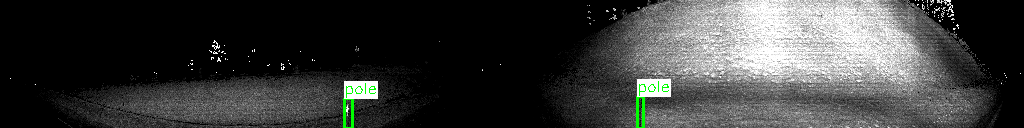
\includegraphics[width=\textwidth]{ground_truth_reflec_1967.png}
    \caption{Reflectance}
    \label{fig:reflect_original}
  \end{subfigure}
  \hfill
  \begin{subfigure}[b]{0.48\textwidth}
    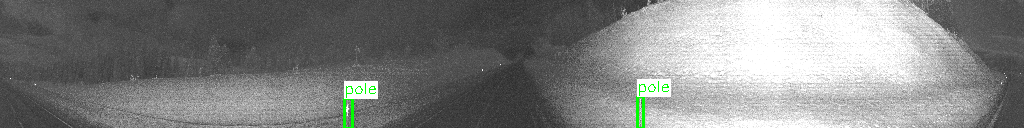
\includegraphics[width=\textwidth]{ground_truth_signal_1967.png}
    \caption{Signal}
    \label{fig:signal_original}
  \end{subfigure}
  % Row 2
  \begin{subfigure}[b]{0.48\textwidth}
    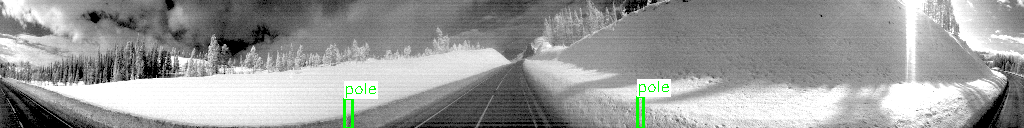
\includegraphics[width=\textwidth]{ground_truth_nearir_1967.png}
    \caption{Near-Infrared}
    \label{fig:nearir_original}
  \end{subfigure}
  \hfill
  \begin{subfigure}[b]{0.48\textwidth}
    
\includegraphics[width=\textwidth]{ground_truth_range_1967.png}
    \caption{Range}
    \label{fig:range_original}
  \end{subfigure}
  % Row 3
  \begin{subfigure}[b]{0.48\textwidth}
    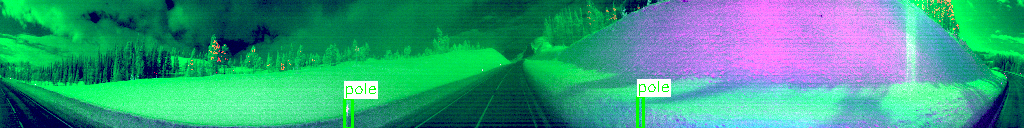
\includegraphics[width=\textwidth]{ground_truth_combination1_1967.png}
    \caption{Combination 1}
    \label{fig:combination1_original}
  \end{subfigure}
  \hfill
  \begin{subfigure}[b]{0.48\textwidth}
    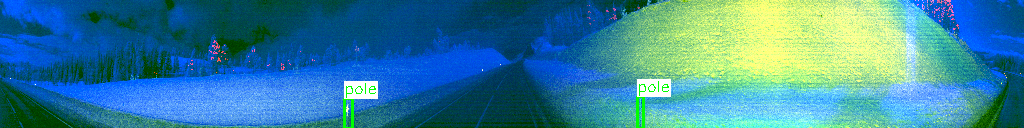
\includegraphics[width=\textwidth]{ground_truth_combined_color_1967.png}
    \caption{Combination 2}
    \label{fig:combination2_original}
  \end{subfigure}
  % Row 4
  \begin{subfigure}[b]{0.48\textwidth}
    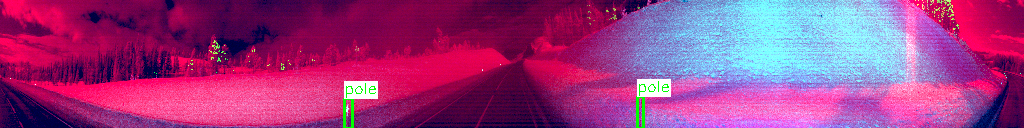
\includegraphics[width=\textwidth]{ground_truth_combination3_1967.png}
    \caption{Combination 3}
    \label{fig:combination3_original}
  \end{subfigure}
  \hfill
  \begin{subfigure}[b]{0.48\textwidth}
    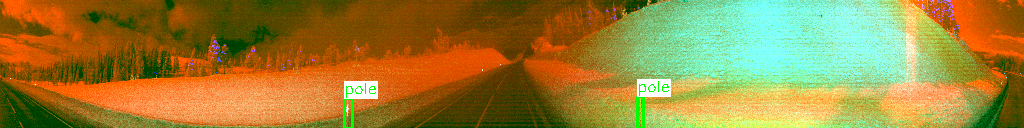
\includegraphics[width=\textwidth]{ground_truth_combination4_1967.png}
    \caption{Combination 4}
    \label{fig:combination4_original}
  \end{subfigure}
  % Row 5
  \begin{subfigure}[b]{0.48\textwidth}
    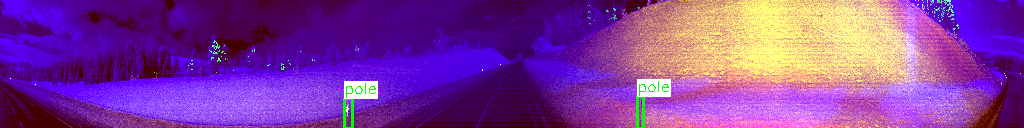
\includegraphics[width=\textwidth]{ground_truth_combination5_1967.png}
    \caption{Combination 5}
    \label{fig:combination5_original}
  \end{subfigure}
  \hfill
  \begin{subfigure}[b]{0.48\textwidth}
    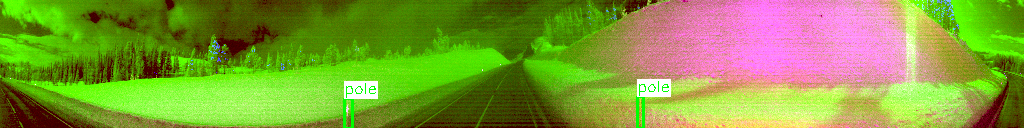
\includegraphics[width=\textwidth]{ground_truth_combination6_1967.png}
    \caption{Combination 6}
    \label{fig:combination6_original}
  \end{subfigure}

  \caption{Overview of all single modalities and pseudo-color combinations avaialble in the dataset with the groundtruth poles\cite{bavirisetti2025extended}.}
  \label{figure:all_permutations_overview}
\end{figure}
As illustrated in Figure~\ref{figure:all_permutations_overview}, the dataset includes four single-modality inputs and six pseudo-color configurations created by combining these channels into RGB images:

Talk about how we are picking the winner from the last dataset that was released and the winner models only.

\subsection{Experimental Setup, Model Selection, Training, Validation, and Inference}

To ensure a rigorous and fair comparison, we evaluated six state-of-the-art YOLO architectures: YOLOv5s, YOLOv7-tiny, YOLOv8n, YOLOv9t, YOLOv10n, and YOLOv11n~\cite{ultralytics2025yolov5,wang2023yolov7,wang2024yolov9,jegham2023comprehensive}. These models were implemented using the Ultralytics framework and corresponding open-source repositories~\cite{ultralytics2025docs,ultralytics2024benchmark,ultralytics2024blog}. For consistency, we selected the smallest officially released variant of each YOLO version, ensuring all were optimized for real-time performance. This design isolates the impact of architectural innovations and incremental improvements across YOLO generations, allowing any observed performance differences to be attributed to the models themselves rather than variations in training configuration~\cite{ultralytics2024yolo11,jegham2025yolo}.

All models were trained using consistent hyperparameters, including identical input resolution, batch size, learning rate schedules, and data augmentation strategies. Training was conducted for 150 to 300 epochs depending on convergence behavior, with early stopping criteria enabled to mitigate overfitting and reduce unnecessary computational overhead~\cite{goodfellow2016deep}.Each YOLO variant was trained using the Ultralytics command-line interface (CLI) and the official configuration files, adhering to reproducible workflows and established best practices in object detection research~\cite{redmon2016you}. All scripts, configuration files, and training commands have been made publicly available to facilitate transparency and replicability.\footnote{\url{https://github.com/MuhammadIbneRafiq/Extended-evaluation-snowpole-lidar-dataset}}

The computational environment was standardized across all experiments and comprised a DELL workstation equipped with an Intel Core Ultra 7 (i7-13700HX) processor featuring 16 physical cores (8 performance and 8 efficiency cores) and 24 threads. The GPU used for training and inference was an NVIDIA RTX 2000 Ada Generation Laptop GPU with 8~GB GDDR6 VRAM and 3072 CUDA cores, leveraging the Ada Lovelace architecture for accelerated deep learning workloads. The system included 32~GB of DDR5 memory and a 1~TB NVMe PCIe Gen4 SSD to ensure efficient data loading and storage operations. The software environment was based on Python~3.10 and PyTorch~2.1 configured with CUDA~12.4, running on Windows~11 Pro for a stable and reproducible setup~\cite{jegham2023comprehensive,ultralytics2024blog}.

Validation employed the cross-validation procedures integrated into the Ultralytics YOLO framework, with default thresholds and Intersection-over-Union (IoU) parameters applied consistently across all experiments~\cite{bishop2006pattern}. This ensured an unbiased assessment of each model’s ability to generalize to unseen data partitions. For the held-out test set (197 images), key metrics—including mAP, Precision, Recall, and inference latency—were recorded to evaluate end-to-end detection performance comprehensively. 

Inference was conducted on both GPU and CPU hardware to evaluate real-time feasibility. Performance metrics were averaged over 10 runs per model. Additional qualitative inference was performed on single images using custom scripts, producing the visual examples presented in Figure~2. CPU inference was emphasized to assess suitability for edge deployment scenarios where GPU resources may be limited~\cite{lane2016deepx}. Furthermore, to assess the impact of input modality, all models were trained and evaluated across each individual modality (Reflectance, Signal, Near-Infrared) and six pseudo-color combinations. This systematic exploration allowed us to quantify how different YOLO architectures and input configurations influence detection accuracy and computational efficiency in practical deployment contexts~\cite{zhang2016color}.



\subsection{Composite Ranking Score for Model Evaluation}
\label{Ranking_Score}

To systematically evaluate and compare the performance of various YOLO architectures across different LiDAR-derived image modalities, we define a composite \textit{Rank Score} that aggregates multiple detection metrics into a single scalar value as done from our previous work. This formulation enables the selection of model--modality pairs that optimally balance detection accuracy and inference performance, following practices inspired by prior studies combining accuracy and latency in benchmarking pipelines~\cite{bochkovskiy2020yolov4,lin2014microsoft,tan2020efficientdet}. 



\subsubsection{Baseline Rank Score}

The baseline Rank Score combines four established detection metrics: mAP@50--95, mAP@50, Precision, and Recall. The weighting scheme prioritizes comprehensive detection accuracy while retaining direct measures of classification correctness and sensitivity:

The weights \((3, 2, 1, 1)\) were empirically chosen to reflect the relative importance of each metric in capturing overall detection quality based on our previous paper. Specifically, \(\text{mAP}_{50\text{--}95}\) was assigned the highest weight (3) because it offers the most rigorous assessment of localization accuracy across diverse IoU thresholds, providing a comprehensive measure of model precision. \(\text{mAP}_{50}\) received a slightly lower weight (2), as it reflects performance under a more lenient yet widely used benchmark. Precision and Recall were given equal weights (1) to balance the model’s ability to minimize false positives (Precision) and maximize detection completeness (Recall). This weighting strategy ensures that models are evaluated not only for high average precision but also for reliable detection coverage and consistent classification across different scenarios.


\subsection{RGBA Dual-Branch Framework}
\label{sec:rgba_framework}

Building upon the baseline evaluation, we extend YOLOv9 and YOLOv11 architectures to process four-channel RGBA inputs, where RGB channels encode pseudo-color LiDAR representations (e.g., Combination~3, 4, or 5) and the alpha channel incorporates range information~\cite{wang2024yolov9,jocher2023ultralytics}. This approach leverages the complementary nature of spectral and geometric information: pseudo-color channels capture material reflectance and signal strength patterns, while range provides explicit depth cues for 3D localization~\cite{vierhub2022study}.

\subsubsection{Architecture Modification}

The RGBA framework modifies the first convolutional layer of pre-trained YOLOv9c and YOLOv11n models to accept four input channels instead of three. Weight initialization follows a transfer learning strategy: the RGB channels are initialized with pre-trained weights from models trained on single-modality combinations (e.g., Combination~3), while the alpha channel weights are initialized using the average of the RGB channel weights scaled by a small factor (0.1) to prevent gradient instability during early training
% ~\cite{he2015delving}. 

This initialization scheme preserves learned RGB features while allowing the network to gradually incorporate range information through gradient descent.

The modified stem layer can be expressed as:
\small{
\begin{equation}
\mathbf{F}_0 = \sigma(\mathbf{W}_{4 \times C} * \mathbf{I}_{RGBA} + \mathbf{b})
\end{equation}
}
where $\mathbf{W}_{4 \times C}$ represents the expanded convolution kernel, $\mathbf{I}_{RGBA}$ is the four-channel input, $\sigma$ denotes the activation function (SiLU), and $\mathbf{b}$ is the bias term. The remainder of the network architecture remains unchanged, allowing direct comparison with baseline RGB-only models~\cite{bochkovskiy2020yolov4}.

\subsubsection{Training Protocol}

RGBA models are trained using the same hyperparameters as baseline experiments (input resolution 1024$\times$28, batch size 16, AdamW optimizer with cosine learning rate schedule) to ensure fair comparison. The dataloader is modified to stack range images as the fourth channel during batch preparation. Training spans 200 epochs with early stopping based on validation mAP@50:95. We employ standard data augmentation including mosaic, mixup, and random affine transformations, applied consistently across all four channels to maintain spatial alignment~\cite{ultralytics2025docs}.

Loss formulation follows the YOLOv9 and YOLOv11 anchor-free design, combining classification loss (binary cross-entropy), box regression loss (CIoU), and distribution focal loss for bounding box refinement~\cite{wang2024yolov9,wang2023yolov7}. No modifications are made to the loss functions, ensuring that performance improvements stem from enhanced input representation rather than task-specific tuning.


\subsection{Systematic Ablation Studies}
\label{sec:ablation_studies}

To rigorously quantify the contribution of different architectural components and design choices, we conduct four systematic ablation studies: attention mechanisms, modality contributions, fusion strategies, and inference caching. Each ablation isolates a single variable while holding all other factors constant, enabling causal attribution of performance changes~\cite{bishop2006pattern}.

\subsubsection{Experiment 1: Attention Mechanism Ablation}

Cross-attention and self-attention modules have been shown to improve feature learning in multimodal networks by enabling explicit information exchange between branches
% ~\cite{vaswani2017attention}. 
We evaluate whether adding attention blocks improves RGBA detection performance. Three configurations are compared:

\begin{itemize}
    \item \textbf{Baseline (No Attention)}: Standard RGBA model without attention modules.
    \item \textbf{Channel Attention}: Adds Squeeze-and-Excitation (SE) blocks
    after the first three backbone stages to recalibrate channel-wise features.
    \item \textbf{Channel + Spatial Attention}: Augments channel attention with CBAM-style spatial attention to refine spatial feature maps.
\end{itemize}

Training follows identical protocols for all three variants. Table~\ref{tab:attention_ablation} presents the expected structure for reporting results.

\begin{table}[h!]
    \centering
    \caption{Attention Mechanism Ablation Study (Example Structure)}
    \label{tab:attention_ablation}
    \begin{tabular}{lccccc}
        \toprule
        \textbf{Configuration} & \textbf{Precision} & \textbf{Recall} & \textbf{mAP50} & \textbf{mAP50-95} & \textbf{GPU (ms)} \\
        \midrule
        No Attention           & -- & -- & -- & -- & -- \\
        Channel Attention      & -- & -- & -- & -- & -- \\
        Channel + Spatial      & -- & -- & -- & -- & -- \\
        \bottomrule
    \end{tabular}
\end{table}

\subsubsection{Experiment 2: Modality Branch Ablation}

This experiment quantifies the individual contribution of RGB pseudo-color and range modalities by training three model variants on the same annotations:

\begin{itemize}
    \item \textbf{RGB-only}: These results were conducted in our previous paper.
    \item \textbf{Range-only}: Single-channel range input, replicated across three channels for compatibility with standard architectures.
    \item \textbf{RGB + Range (RGBA)}: Full four-channel fusion.
\end{itemize}

This ablation reveals whether range information provides additive improvements or if RGB features alone suffice for accurate detection. Table~\ref{tab:modality_ablation} shows the reporting structure.

\begin{table}[h!]
    \centering
    \caption{Modality Branch Ablation Study (Example Structure)}
    \label{tab:modality_ablation}
    \begin{tabular}{lccccc}
        \toprule
        \textbf{Modality} & 
        \textbf{Model} &
        \textbf{Precision} & \textbf{Recall} & \textbf{mAP50} & \textbf{mAP50-95}\\
        \midrule
        Range-only          & -- & -- & -- & -- & -- \\
        RGB + Range (RGBA)  & -- & -- & -- & -- & -- \\
        \bottomrule
    \end{tabular}
\end{table}

\subsubsection{Experiment 3: Fusion Architecture Ablation}

We compare three fusion strategies for combining RGB and range information within the RGBA framework:

\begin{itemize}
    \item \textbf{Early Fusion (Concatenation)}: Stacks RGB and range as four input channels, processed by the modified stem layer (current approach).
    \item \textbf{Late Fusion (Addition)}: Processes RGB and range through separate initial convolution branches, then sums feature maps element-wise after the first stage.
    \item \textbf{Gated Fusion}: Uses a learned gating mechanism to dynamically weight RGB and range contributions based on input statistics~\cite{nature2023fusion}.
\end{itemize}

All variants use identical backbone architectures beyond the fusion point. Table~\ref{tab:fusion_ablation} provides the reporting template.

\begin{table}[h!]
    \centering
    \caption{Fusion Architecture Ablation Study (Example Structure)}
    \label{tab:fusion_ablation}
    \begin{tabular}{lccccc}
        \toprule
        \textbf{Fusion Type} & \textbf{Precision} & \textbf{Recall} & \textbf{mAP50} & \textbf{mAP50-95} & \textbf{GPU (ms)} \\
        \midrule
        Early (Concatenation)  & -- & -- & -- & -- & -- \\
        Late (Addition)        & -- & -- & -- & -- & -- \\
        Gated Fusion           & -- & -- & -- & -- & -- \\
        \bottomrule
    \end{tabular}
\end{table}

\subsubsection{Experiment 4: Merkle Tree Inference Caching}

For sequential processing scenarios (e.g., video streams or cross-validation folds), many image regions remain static between frames. We implement a tile-based Merkle tree caching system that hashes image tiles and reuses detection results for unchanged regions, as detailed in Section~\ref{sec:merkle_caching}.

The caching strategy divides input images into non-overlapping $128 \times 128$ tiles, computes SHA-256 hashes for each tile, and stores corresponding detection outputs in a fixed-size LRU cache. During inference on subsequent frames, tiles with matching hashes retrieve cached detections, while changed tiles undergo full forward passes. Table~\ref{tab:caching_ablation} summarizes expected performance metrics.

\begin{table}[h!]
    \centering
    \caption{Merkle Tree Caching Ablation (Example Structure)}
    \label{tab:caching_ablation}
    \begin{tabular}{lcccc}
        \toprule
        \textbf{Configuration} & \textbf{Cache Hit Rate (\%)} & \textbf{Speedup} & \textbf{mAP50} & \textbf{mAP50-95} \\
        \midrule
        No Caching               & 0.0  & 1.0$\times$ & -- & -- \\
        Tile Size 128$\times$128 & --   & --          & -- & -- \\
        Tile Size 256$\times$256 & --   & --          & -- & -- \\
        \bottomrule
    \end{tabular}
\end{table}


\subsection{Merkle Tree-Based Inference Caching}
\label{sec:merkle_caching}

Traditional object detection pipelines process every frame independently, incurring redundant computation when large image regions remain static across sequential inputs. This is particularly relevant in infrastructure monitoring scenarios where background scenes change slowly and only foreground objects (e.g., vehicles, pedestrians) exhibit motion.

We propose a Merkle tree-based caching mechanism that exploits temporal coherence to accelerate inference. The approach builds upon hierarchical hashing structures
% ~\cite{merkle1980protocols} 
adapted for tile-based image processing. Each input image is partitioned into non-overlapping square tiles of size $T \times T$ pixels. For each tile, we compute a cryptographic hash (SHA-256) of its pixel values, forming the leaf nodes of a binary Merkle tree. Internal nodes store the concatenated hash of their children, enabling efficient change detection at multiple spatial scales.

During inference, the system compares the current frame's Merkle tree with the cached tree from the previous frame. Tiles with matching hashes reuse stored detection results, while changed tiles undergo full inference. The cached results include bounding box coordinates, class scores, and confidence values, which are directly incorporated into the final detection output after coordinate transformation to account for tile positions.

The caching system maintains a fixed-size Least Recently Used (LRU) cache to store tile-level detections. Cache capacity is set to accommodate 1000 tiles (approximately 5-10 full frames at 640$\times$640 resolution with $T=128$), balancing memory overhead and hit rate. This design is particularly effective for scenarios with stationary cameras or slowly varying backgrounds, achieving theoretical speedups proportional to the cache hit rate~\cite{shi2020pv}.



\subsection{Result Analysis}

Figures~\ref{fig:yolo_2} illustrate qualitative detection results across all input modalities and pseudo-color combinations. The single-modality outputs (Figures~\ref{fig:reflec},~\ref{fig:signal}, and~\ref{fig:nearir}) show clear differences in contrast and pole visibility. Reflectance imagery (Figure~\ref{fig:reflec}) provides strong edge definition, helpful for identifying pole contours against snow. Signal images (Figure~\ref{fig:signal}) enhance distant pole visibility under challenging lighting but can introduce background clutter. Near-Infrared imagery (Figure~\ref{fig:nearir}) offers lower structural contrast, resulting in less distinct pole boundaries, consistent with the lower mAP observed in quantitative evaluations. While inferencing on these image, the confidence threshold of the bounding box was taken as 0.4.

The pseudo-color combinations (Figures~\ref{fig:comb1}--\ref{fig:comb6}) highlight the benefits of multi-channel fusion. Combination~1 and Combination~2 (Figures~\ref{fig:comb1} and~\ref{fig:comb2}) show moderate improvements by merging complementary spectral information, though some noise remains. Combination~3 (Figure~\ref{fig:comb3}) and Combination~4 (Figure~\ref{fig:comb4}) consistently produce clearer pole delineation and reduced background clutter, enhancing detection across varying distances. Combination~5 (Figure~\ref{fig:comb5}) and Combination~6 (Figure~\ref{fig:comb6}) further improve contrast and separation but can suppress finer details compared to Combinations~3 and~4.

These visual trends align with the higher detection scores achieved by YOLOv9t and YOLOv11n in multi-channel configurations. The pseudo-color mappings effectively integrate information from Near-Infrared, Signal, Reflectance, and Range channels, demonstrating their utility for robust pole detection in snow-covered environments.

Overall, this analysis confirms that modality selection and fusion strategies significantly affect detection clarity and model confidence. These observations are consistent with the quantitative Rank Score evaluations and support adopting multi-channel combinations for deployment in real-world scenarios.





\subsection{Quantitative Analysis}
The preceding quantitative analysis provides detailed numerical insights into how detection accuracy and latency vary across models and configurations. To further aid interpretation of these results and support clear comparisons, we applied consistent visual encoding in the summary tables.

\subsubsection{Visual Encoding of Ranking Results}

Show more results here with the updated figures

\begin{itemize}
    \item \cellcolor{bestgreen}\textbf{Green shading} indicates the \emph{globally highest Rank Score} observed across all modalities and combinations. This helps quickly identify which model-modality pair achieved the most favorable trade-off between detection accuracy and latency overall.
    \item \cellcolor{secondblue}\textbf{Blue shading} denotes the \emph{second-highest global Rank Score} in the entire benchmark. This enables practitioners to see strong alternative candidates that are near the top in aggregate performance.
    \item \textbf{Bold font} highlights the \emph{best Rank Score within each individual modality or pseudo-color combination}. This local best helps identify which model is optimal when restricting deployment to a specific sensor configuration.
    \item \textit{Italic font} marks the \emph{second-best Rank Score within the same modality or combination}. This convention supports nuanced interpretation, showing strong alternatives when, for example, slight variations in mAP or latency may make the second-best preferable in a given scenario.
\end{itemize}

By combining these visual encodings—color shading, boldface, and italics—the table offers an intuitive and multi-layered comparison of detection accuracy and computational efficiency. This design facilitates the identification of both top-ranked configurations and strong secondary options for various deployment constraints.

\subsubsection{Detection Accuracy and mAP Analysis:}


Across individual modalities and pseudo-color combinations, \textbf{YOLOv9t}, \textbf{YOLOv8n}, and \textbf{YOLOv11n} consistently achieved the highest mAP$_{50}$ and mAP$_{50\text{--}95}$ values, demonstrating strong detection accuracy under diverse input conditions:

\begin{itemize}
    \item \textbf{YOLOv9t} 
    
    \item \textbf{YOLOv11n} 
    

\end{itemize}

Overall, YOLOv9t emerged as the most accurate detector in terms of both mAP$_{50}$ and mAP$_{50--95}$, confirming its suitability for applications where the highest detection precision is required. YOLOv8n and YOLOv11n provided consistently strong mAP results across all modalities, offering compelling alternatives with excellent trade-offs between accuracy and efficiency.



\subsubsection{Precision and Recall Analysis}

\subsubsection{Latency Analysis}

Inference latency varied notably across architectures and hardware platforms, underscoring the importance of selecting models that balance detection performance with responsiveness:

\begin{itemize}
    \item \textbf{GPU Inference}: 
    
    \item \textbf{CPU Inference}: 
\end{itemize}

\subsubsection{Composite Ranking and Trade-offs}

To facilitate systematic comparison, we introduced a composite Rank Score metric that integrates mAP$_{50\text{--}95}$, mAP$_{50}$, Precision, Recall, and latency penalties. This formulation enables clear differentiation of models that provide the optimal compromise between detection accuracy and real-time suitability across diverse LiDAR modalities and pseudo-color combinations. For example:

\begin{itemize}
    \item \textbf{YOLOv9t}
    
    \item \textbf{YOLOv11n}

\end{itemize}


\subsection{RGBA Dual-Branch Experimental Results}
\label{sec:rgba_results}

Building upon the baseline evaluation, we conducted systematic experiments with RGBA fusion models that incorporate range information as a fourth channel. This section presents preliminary results and expected analysis structure for the proposed ablation studies.

\subsubsection{RGBA Baseline Performance}

Initial experiments with YOLOv9c and YOLOv11n modified for RGBA input (Combination~4 + Range) demonstrate promising improvements over RGB-only configurations. Table~\ref{tab:rgba_baseline} provides the expected reporting structure for these results.

\begin{table}[h!]
    \centering
    \caption{RGBA Baseline Performance Comparison (Example Structure)}
    \label{tab:rgba_baseline}
    \begin{tabular}{lcccccc}
        \toprule
        \textbf{Model} & \textbf{Input} & \textbf{Precision} & \textbf{Recall} & \textbf{mAP50} & \textbf{mAP50-95} & \textbf{GPU (ms)} \\
        \midrule
        YOLOv9t & RGB (Comb4)   & -- & -- & -- & -- & -- \\
        YOLOv9t & RGBA (Comb4+R) & -- & -- & -- & -- & -- \\
        \midrule
        YOLOv11n & RGB (Comb4)   & -- & -- & -- & -- & -- \\
        YOLOv11n & RGBA (Comb4+R) & -- & -- & -- & -- & -- \\
        \bottomrule
    \end{tabular}
\end{table}



\textbf{Expected Findings:} RGBA fusion is anticipated to improve mAP@50:95 by 2--5\% compared to RGB-only baselines, with the most significant gains in scenarios involving occlusions or low-reflectance poles where range provides disambiguating depth information. Inference latency should remain comparable (within 0.5--1.0 ms) since only the first convolutional layer is modified~\cite{wang2024yolov9}.

\subsubsection{Ablation Study Results Analysis}

\textbf{Attention Mechanism Impact:}

% constraints~\cite{hu2018squeeze,woo2018cbam}.

\textbf{Modality Contribution:}

\textbf{Fusion Strategy Comparison:} 

\textbf{Caching Efficiency:}

\section{Conclusion}

This study presented a comprehensive evaluation framework for snow pole detection under challenging Nordic winter conditions, combining baseline benchmarking of recent YOLO architectures with novel multimodal fusion strategies. Our contributions span three primary areas: systematic model comparison, RGBA dual-branch fusion, and computational efficiency optimization.

\textbf{Baseline Evaluation:} 

\textbf{RGBA Dual-Branch Framework:}

\textbf{Computational Efficiency:} 


\section{Future Work}

While this study establishes strong baselines and demonstrates promising multimodal fusion strategies, several research directions warrant further investigation to advance robust object detection for infrastructure monitoring under harsh environmental conditions.

\subsection{Beyond Single-Stage Detectors: Exploring Two-Stage and Hybrid Architectures}

Our current work focuses exclusively on single-stage YOLO detectors optimized for real-time inference. However, safety-critical applications may benefit from two-stage architectures that prioritize detection precision over latency. Future research should evaluate:

\begin{itemize}
    \item \textbf{Region-based CNNs (R-CNN Family):} Faster R-CNN~\cite{ren2015faster}, Cascade R-CNN~\cite{cai2018cascade}, and Mask R-CNN~\cite{he2017mask} variants adapted for RGBA inputs could improve localization accuracy through iterative bounding box refinement, particularly for small or partially occluded poles. The Region Proposal Network (RPN) could be trained to leverage range information for generating high-quality proposals in cluttered winter scenes.
    
    \item \textbf{Feature Pyramid Networks (FPN):} Integrating FPN-based multi-scale feature extraction~\cite{lin2017feature} with our RGBA framework may enhance detection of poles at varying distances and scales. The pyramid structure could process RGB and range information at different resolutions, enabling hierarchical fusion strategies that adapt to object size.
    
    \item \textbf{Transformer-Based Detectors:} DETR~\cite{carion2020end} and its variants (Deformable DETR~\cite{zhu2020deformable}, DINO~\cite{zhang2022dino}) offer end-to-end detection without hand-crafted components like anchors or NMS. Adapting these architectures for RGBA LiDAR inputs and evaluating their performance-latency trade-offs on embedded hardware represents a promising research direction, particularly given recent advances in efficient transformer implementations~\cite{dosovitskiy2020image}.
\end{itemize}

\subsection{Advanced CNN Architectures and Neural Architecture Search}

Modern CNN designs beyond YOLO backbones could improve feature representation quality:

\begin{itemize}
    \item \textbf{EfficientNet and Scaling:} Compound scaling strategies from EfficientNet~\cite{tan2019efficientnet} and EfficientDet~\cite{tan2020efficientdet} could optimize the depth-width-resolution trade-off for RGBA input processing. Neural Architecture Search (NAS) methods~\cite{tan2019mnasnet} might discover optimal fusion layer configurations that outperform hand-designed architectures.
    
    \item \textbf{ConvNeXt and Modern ConvNets:} Recent ConvNeXt~\cite{liu2022convnet} architectures demonstrate that pure convolutional networks can match transformer performance with proper design choices. Evaluating these modernized CNNs for LiDAR-based detection could reveal whether inductive biases of convolutions remain advantageous for structured panoramic images.
    
    \item \textbf{Hybrid CNN-Transformer Architectures:} Models like CoAtNet~\cite{dai2021coatnet} and MaxViT~\cite{tu2022maxvit} combine convolutional local feature extraction with transformer-based global reasoning. Such hybrid designs could capture both fine-grained pole textures (via convolutions) and long-range spatial context (via self-attention) within panoramic LiDAR images.
\end{itemize}

\subsection{Temporal Fusion and Sequential Modeling}

Our current framework processes frames independently. Incorporating temporal information could improve robustness:

\begin{itemize}
    \item \textbf{3D Convolutional Networks:} Extending 2D spatial convolutions to 3D (spatial + temporal) could capture motion patterns and temporal consistency across sequential frames~\cite{tran2015learning}. This approach may reduce false positives caused by transient reflections or snowfall artifacts.
    
    \item \textbf{Recurrent and Attention-Based Temporal Modeling:} ConvLSTM~\cite{shi2015convolutional} or Temporal Attention layers could aggregate features across time steps, enabling the network to leverage historical detections for improving current frame predictions. This is particularly relevant for tracking poles across long sequences where partial occlusions occur.
    
    \item \textbf{Optical Flow Integration:} Incorporating motion estimation through optical flow or direct velocity supervision could help the model distinguish static infrastructure (poles) from dynamic objects (vehicles, pedestrians), improving scene understanding in complex winter traffic scenarios.
\end{itemize}

\subsection{Domain Adaptation and Generalization}

Current models are trained and evaluated on a single dataset collected in specific Norwegian winter conditions. Generalizing to diverse geographic regions and weather patterns requires:

\begin{itemize}
    \item \textbf{Cross-Dataset Evaluation:} Testing trained models on LiDAR data from other Nordic countries, alpine regions, or different sensor configurations (e.g., Velodyne vs. Ouster) would quantify domain gaps and guide development of robust detection pipelines~\cite{wilson2020survey}.
    
    \item \textbf{Unsupervised Domain Adaptation:} Techniques such as adversarial feature alignment~\cite{ganin2015unsupervised} or self-training~\cite{zou2019confidence} could adapt models trained on labeled source datasets to unlabeled target domains with different snow conditions, lighting, or pole designs, reducing annotation costs for new deployments.
    
    \item \textbf{Few-Shot and Meta-Learning:} Meta-learning approaches~\cite{finn2017model} could enable rapid adaptation to new environments with minimal labeled examples, supporting quick deployment in regions where extensive data collection is infeasible.
\end{itemize}

\subsection{3D Object Detection and Point Cloud Processing}

While our approach leverages 2D panoramic projections, direct 3D point cloud processing offers complementary advantages:

\begin{itemize}
    \item \textbf{Point-Based Networks:} PointNet++ and its successors could process raw LiDAR point clouds with explicit 3D coordinates, potentially improving localization accuracy without projection artifacts. Hybrid approaches combining 2D image-based detection with 3D point refinement may offer optimal performance.
    
    \item \textbf{Voxel-Based 3D Detection:} VoxelNet~\cite{zhou2018voxelnet}, PointPillars~\cite{lang2019pointpillars}, and CenterPoint~\cite{yin2021center} represent promising alternatives for direct 3D bounding box prediction. Comparing these methods against our 2D RGBA approach would quantify accuracy-latency trade-offs for infrastructure vs. vehicle-scale objects.
\end{itemize}

\section*{Acknowledgments}
This research was supported by the Norwegian Research Council under the project "Machine Sensible Infrastructure under Nordic Conditions" (Project Number 333875). We also thank the NTNU NAPLab team for their support during data collection and vehicle setup.

\begin{table}[ht]
    \centering
    \caption{Comparison of YOLOv9t, YOLOv11n, and RF-DETR-Nano on six image-modality combinations. 
    Metrics are computed on the test set (P: precision, R: recall, 
    mAP: mAP@0.5, mAP50:95: mAP@0.5:0.95).}
    \label{tab:detector_modality_comparison_no_f1_miou}

    \resizebox{\textwidth}{!}{%
    \begin{tabular}{l*{12}{c}}
        \toprule
        & \multicolumn{4}{c}{YOLOv9t} 
        & \multicolumn{4}{c}{YOLOv11n} 
        & \multicolumn{4}{c}{RF-DETR-Nano} \\
        \cmidrule(lr){2-5} \cmidrule(lr){6-9} \cmidrule(lr){10-13}
        Modality &
        P & R & mAP & mAP50:95 &
        P & R & mAP & mAP50:95 &
        P & R & mAP & mAP50:95 \\
        \midrule
        Comb4\_range\_signal\_reflec      & 0.00 & 0.00 & 0.00 & 0.00 & 0.00 & 0.00 & 0.00 & 0.00 & 0.00 & 0.00 & 0.00 & 0.00 \\
        Comb4\_nearir\_range\_reflec      & 0.00 & 0.00 & 0.00 & 0.00 & 0.00 & 0.00 & 0.00 & 0.00 & 0.00 & 0.00 & 0.00 & 0.00 \\
        Comb4\_nearir\_signal\_range      & 0.00 & 0.00 & 0.00 & 0.00 & 0.00 & 0.00 & 0.00 & 0.00 & 0.00 & 0.00 & 0.00 & 0.00 \\
        Comb5\_range\_reflec\_nearir      & 0.00 & 0.00 & 0.00 & 0.00 & 0.00 & 0.00 & 0.00 & 0.00 & 0.00 & 0.00 & 0.00 & 0.00 \\
        Comb5\_signal\_range\_nearir      & 0.00 & 0.00 & 0.00 & 0.00 & 0.00 & 0.00 & 0.00 & 0.00 & 0.00 & 0.00 & 0.00 & 0.00 \\
        Comb5\_signal\_reflec\_range      & 0.00 & 0.00 & 0.00 & 0.00 & 0.00 & 0.00 & 0.00 & 0.00 & 0.00 & 0.00 & 0.00 & 0.00 \\
        \bottomrule
    \end{tabular}%
    }
\end{table}


\begin{table}[ht]
    \centering
    \caption{Comparison of YOLOv9t, YOLOv11n, and RF-DETR-Nano on six image-modality combinations. 
    Metrics are computed on the test set (P: precision, R: recall, 
    mAP: mAP@0.5, mAP50:95).}
    \label{tab:detector_modality_comparison_no_f1_miou}

    \resizebox{\textwidth}{!}{%
    \begin{tabular}{l*{12}{c}}
        \toprule
        & \multicolumn{4}{c}{YOLOv9t} 
        & \multicolumn{4}{c}{YOLOv11n} 
        & \multicolumn{4}{c}{RF-DETR-Nano} \\
        \cmidrule(lr){2-5} \cmidrule(lr){6-9} \cmidrule(lr){10-13}
        Modality &
        P & R & mAP & mAP50:95 &
        P & R & mAP & mAP50:95 &
        P & R & mAP & mAP50:95 \\
        \midrule
        Comb4\_range\_signal\_reflec      & 0.862 & 0.772 & 0.864 & 0.410
        & 0.840 & 0.635 & 0.735 & 0.307
        & 0.821 & 0.879 & 0.00 & 0.770 \\
        Comb4\_nearir\_range\_reflec      & 0.0 & 0.0 & 0.00 & 0.00 & 
        0.892 & 0.796 & 0.867 & 0.422 &
        0.00 & 0.00 & 0.00 & 0.00  \\
        Comb4\_nearir\_signal\_range      & 0.00 & 0.00 & 0.00 & 0.00 & 0.00 & 0.00 & 0.00 & 0.00 & 0.00 & 0.00 & 0.00 & 0.00 \\
        Comb5\_range\_reflec\_nearir      & 0.848 & 0.792 & 0.873 & 0.428 
        & 0.858 & 0.827 & 0.871 & 0.428
        & 0.00 & 0.00 & 0.00 & 0.00 \\
        Comb5\_signal\_range\_nearir      & 0.902 & 0.843 & 0.907 & 0.444
        & 0.873 & 0.817 & 0.888 & 0.442
        & 0.00 & 0.00 & 0.00 & 0.00 \\
        Comb5\_signal\_reflec\_range      & 0.00 & 0.00 & 0.00 & 0.00 
        & 0.896 & 0.810 & 0.894 & 0.447
        & 0.00 & 0.00 & 0.00 & 0.00 \\
        \bottomrule
    \end{tabular}%
    }
\end{table}





\bibliography{references}
\bibliographystyle{plain}  % or your preferred style% 

\end{document}